\section{Planteamiento del problema}

\begin{frame}{Estado actual del Instituto Andrés Barbero}

%\begin{figure}
%    \begin{subfigure}[b]{.6\linewidth}
%        \centering
%        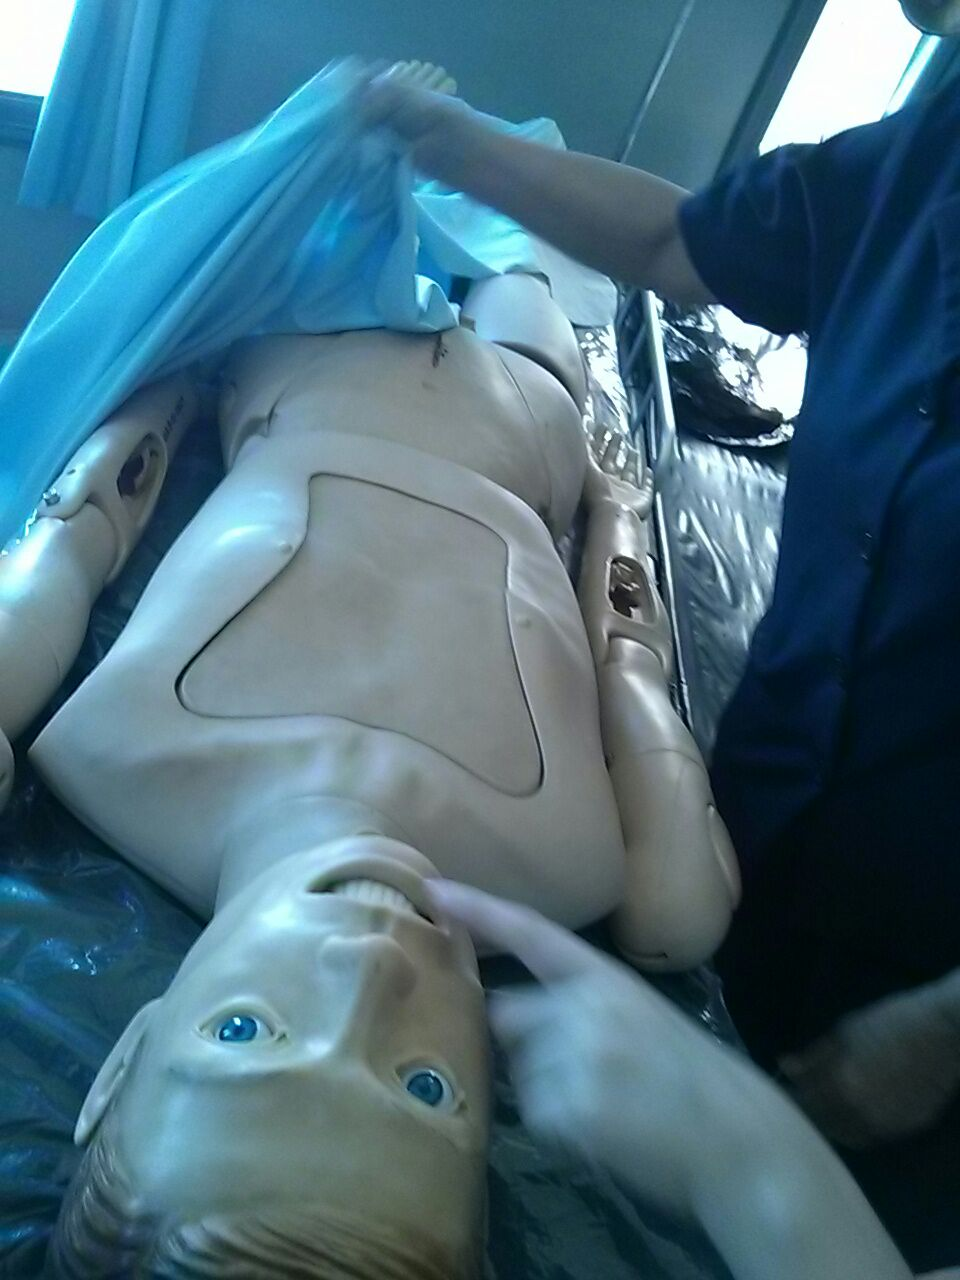
\includegraphics[height=3cm]{../problema/iab_sala_3.jpg}
%        \caption{Tiempo por tipo de actividad}
%    \end{subfigure}

    
%    \begin{subfigure}[b]{.6\linewidth}
	\begin{enumerate}[<+->]
	\item Prácticas en laboratorio
	\item Prácticas en hospitales o prácticas de campo
	\end{enumerate}
%	\end{subfigure}
%\end{figure}
\end{frame}

\begin{frame}{Problemas actuales del Instituto Andrés Barbero}
	\begin{enumerate}[<+->]
	\item Falta de preparación de los alumnos
	\item Definición de un protocolo de comunicación
	\item Nerviosismo ante la primera práctica
	\item Alta carga horaria de los trabajos prácticos
	\item Reducida carga horaria para el estudio de las materias teóricas
	\item Poca flexibilidad de los profesores
	\item Falta de materiales actualizados para los profesores
	\item Problemas de transporte
	\item Falta de preparación para las prácticas
	\item Alta cantidad de alumnos
	\end{enumerate}
\end{frame}

\begin{frame}{Propuesta de solución}
	\begin{enumerate}[<+->]
	\item Evaluación
	\item Progreso
	\item Tiempo de práctica
	\item Factor psicológico
	\item Ubicuidad
	\item Realismo
	\item Enfoque individual
	\end{enumerate}
\end{frame}

%\begin{frame}{Requerimientos de la solución}\end{frame}

\begin{frame}{Alcance de la solución (I)}
	Factores limitantes.
	\begin{enumerate}[<+->]
	\item Limitaciones técnicas
	\item Importancia de representación
	\item Facilidad de realización
	\end{enumerate}
\end{frame}

\begin{frame}{Alcance de la solución (II)}
	Hipótesis.
	\begin{enumerate}[<+->]
	\item Comando de voz con interfaz
	\item Extracción uniforme de elementos
	\item Acciones de bioseguridad
	\item Representación iconográfica
	\item Factores limitantes
	\item Falta de pistas
	\item Ubicuidad
	\end{enumerate}
\end{frame}

\begin{frame}{Alcance de la solución (III)}
	Decisiones de diseño.
	\begin{enumerate}[<+->]
	\item Acciones por interfaz de usuario
	\item Simulación integra de pasos
	\end{enumerate}
\end{frame}
